\documentclass{beamer}
%\documentclass[handout,numbers]{beamer}
%\documentclass[handout,draft]{beamer}
%\includeonlyframes{current}
\usepackage{pgfpages}
\usepackage[english]{babel}
%\usepackage[latin1]{inputenc}
%\usepackage{times}
%\usepackage[T1]{fontenc}
\usepackage{versions}
\excludeversion{TOKEEPSECRET}
\newcommand{\OPT}{\mbox{\rm OPT}}
\newcommand{\A}{\mathcal{A}}
\newcommand{\Ss}{\mathcal{S}}

\mode<handout>{
  \setbeameroption{show notes}
  \pgfpagesuselayout{4 on 1}[letterpaper,border shrink=5mm,landscape]
  % instead of   \pgfpagelayout{4 on 1}[border shrink=5mm,landscape]
  \setbeamercolor{background canvas}{bg=black!5}
}
\mode<presentation>
{
  \usetheme{Warsaw}
  \setbeamercovered{transparent}
  \setbeamertemplate{footline}{\hfill\insertframenumber/\inserttotalframenumber} 
  \AtBeginSection[]
  {
    \begin{frame}<beamer>
      \frametitle{Outline}
      \tableofcontents[currentsection]
    \end{frame}
  }
}


\title[From Fine Analysis to Instance Optimality] 
{From Fine Analysis to Instance Optimality}
\author{J{\'e}r{\'e}my Barbay}

\institute[Universidad de Chile] 
{
  Departmento de Ciencias de la Computacion\\
  Universidad de Chile
}

\date{}
\subject{Talks}


% If you wish to uncover everything in a step-wise fashion, uncomment
% the following command: 
%\beamerdefaultoverlayspecification{<+->}


\begin{document}

\begin{frame}
  \titlepage
\end{frame}

\begin{frame}
  \frametitle{Outline}
  \tableofcontents
  % You might wish to add the option [pausesections]
\end{frame}


\section{The Convex Hull Paradox}

\begin{frame}<presentation>
  \frametitle{The Planar Convex Hull}
  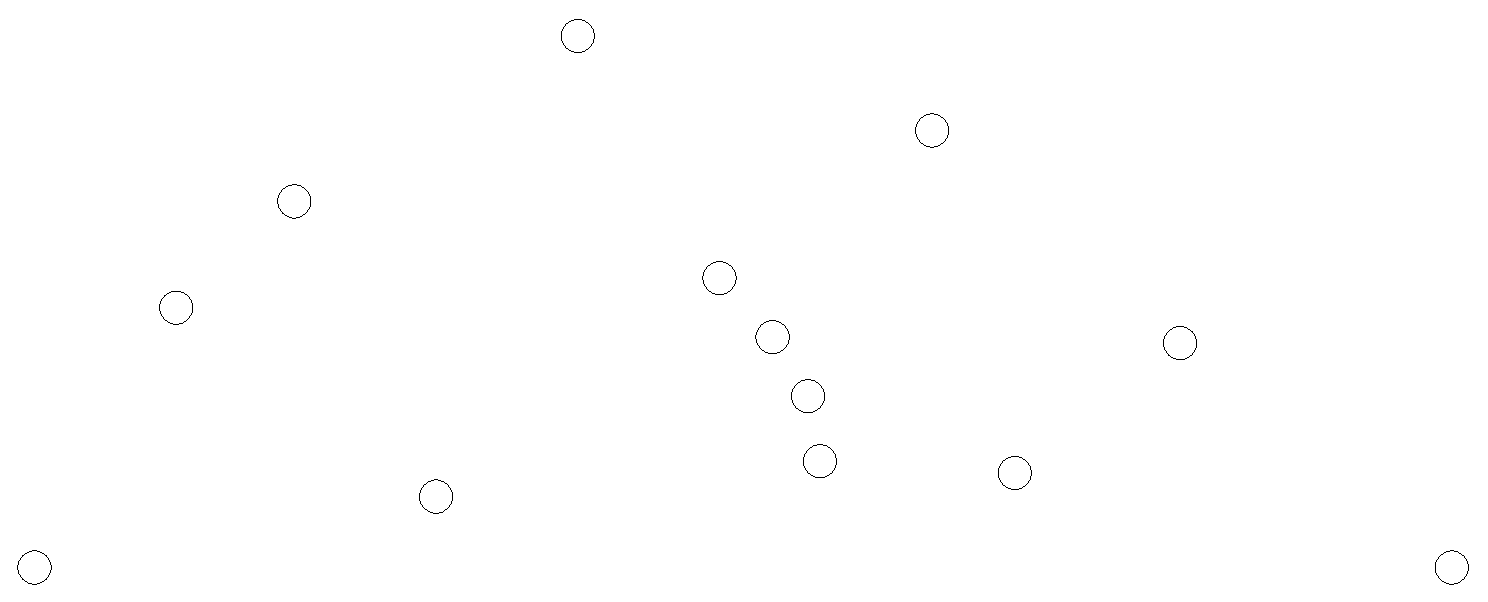
\includegraphics[width=\textwidth]{points}
  \begin{itemize}
  \item Can one of you define it?
  \item What is the best complexity known for it?
  \end{itemize}
\end{frame}


\subsection{$O(n\lg n)$}
\begin{frame}
  \frametitle{2d Convex Hull in $O(n\lg n)$}
  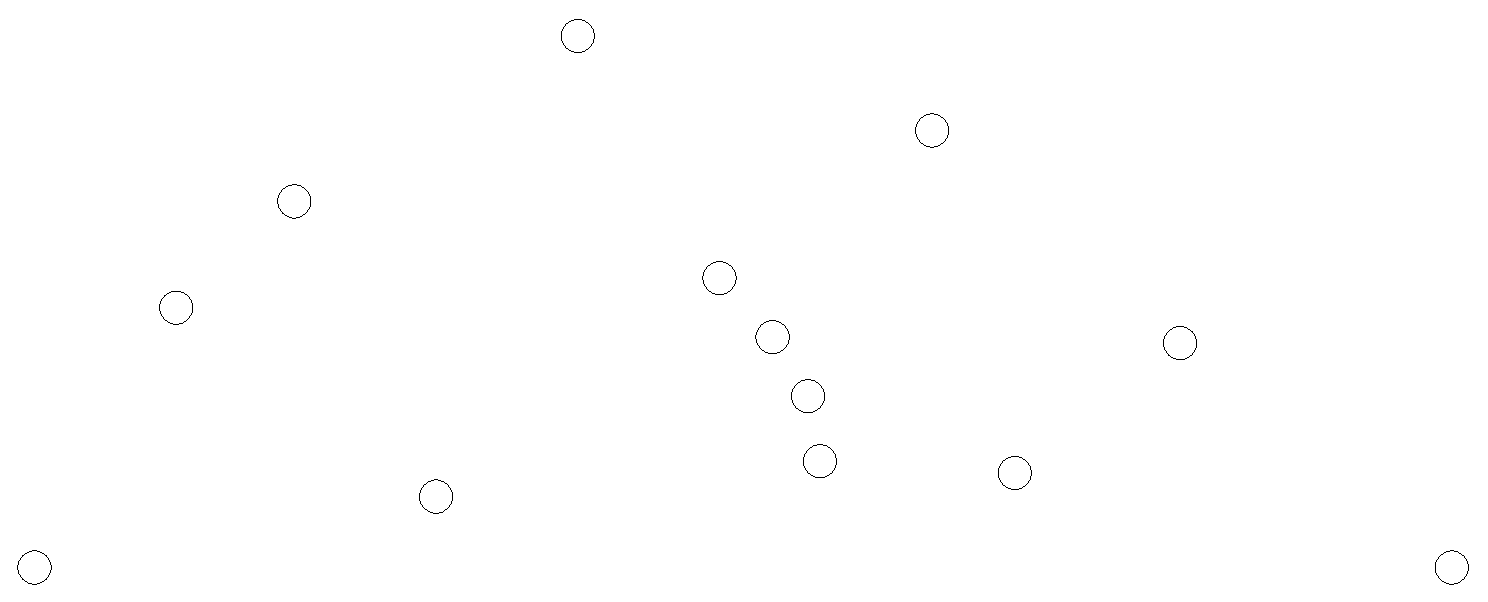
\includegraphics[width=\textwidth]{points}
  \begin{enumerate}
  \item Sort the points by $x$-coordinates;
  \item Scan them, backtracking if necessary.
  \end{enumerate}
\end{frame}



\subsection{$O(nh)$}
\begin{frame}
  \frametitle{2d Convex Hull in $O(nh)$}
  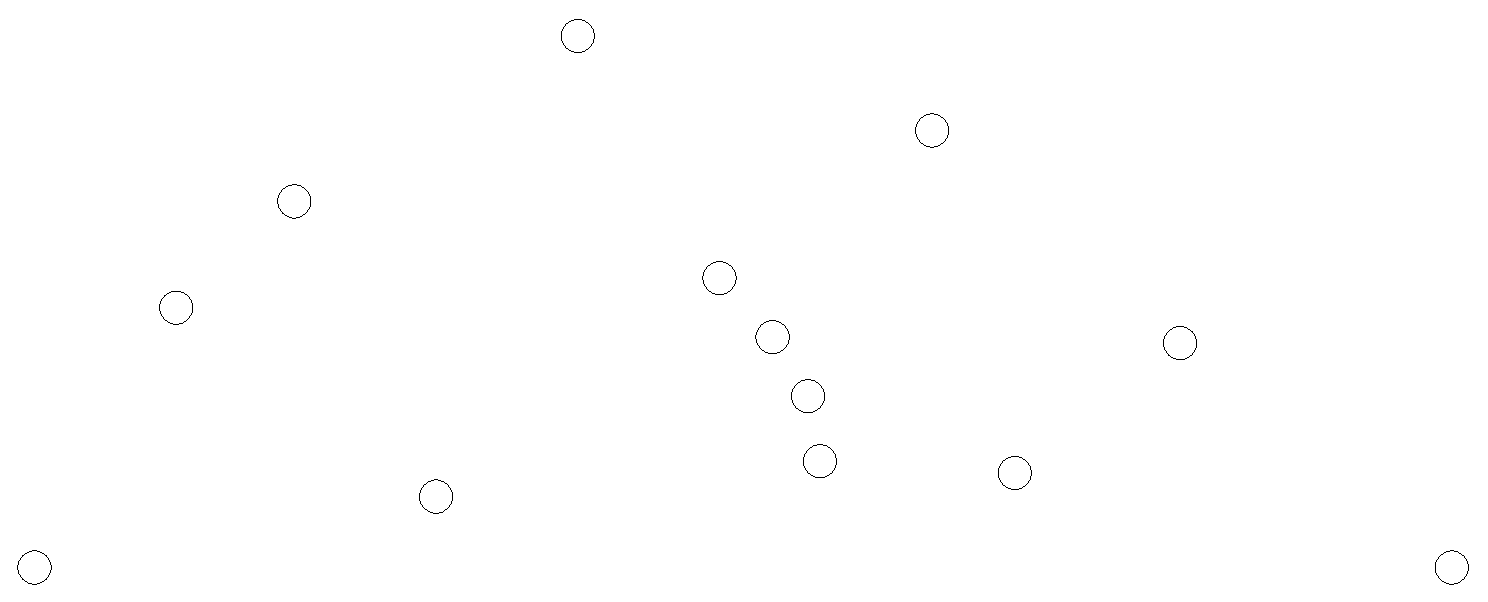
\includegraphics[width=\textwidth]{points}
  \begin{enumerate}
  \item Find the left-most point
  \item Compute the $n-1$ slopes with the other points
  \item Choose the highest slope
  \item Iterate 
  \end{enumerate}
\end{frame}


\subsection{Worst Case Complexity?}

\begin{frame}
  \frametitle{Worst case Complexity of 2d Convex Hull}
  \begin{itemize}
  \item Question ill-defined: the worst case over what?
    \begin{itemize}
    \item all instances of fixed size $n$?
    \item all instances of fixed input size $n$ and output size $h$?
    \end{itemize}
  \item For each we have distinct lower bounds:
    \begin{itemize}
    \item $\Omega(n\lg n)$, which is tight; and
    \item $\Omega(n\lg h)$, which is \alert{not} tight!
    \end{itemize}
  \item So what is the complexity of 2d convex hull?
  \end{itemize}
\end{frame}



\section{Fine analysis of the convex hull}

\subsection{$O(n\lg h)$ in 2D}
\begin{frame}
  \frametitle{2d Convex Hull in $O(n\lg h)$ in 2D}
  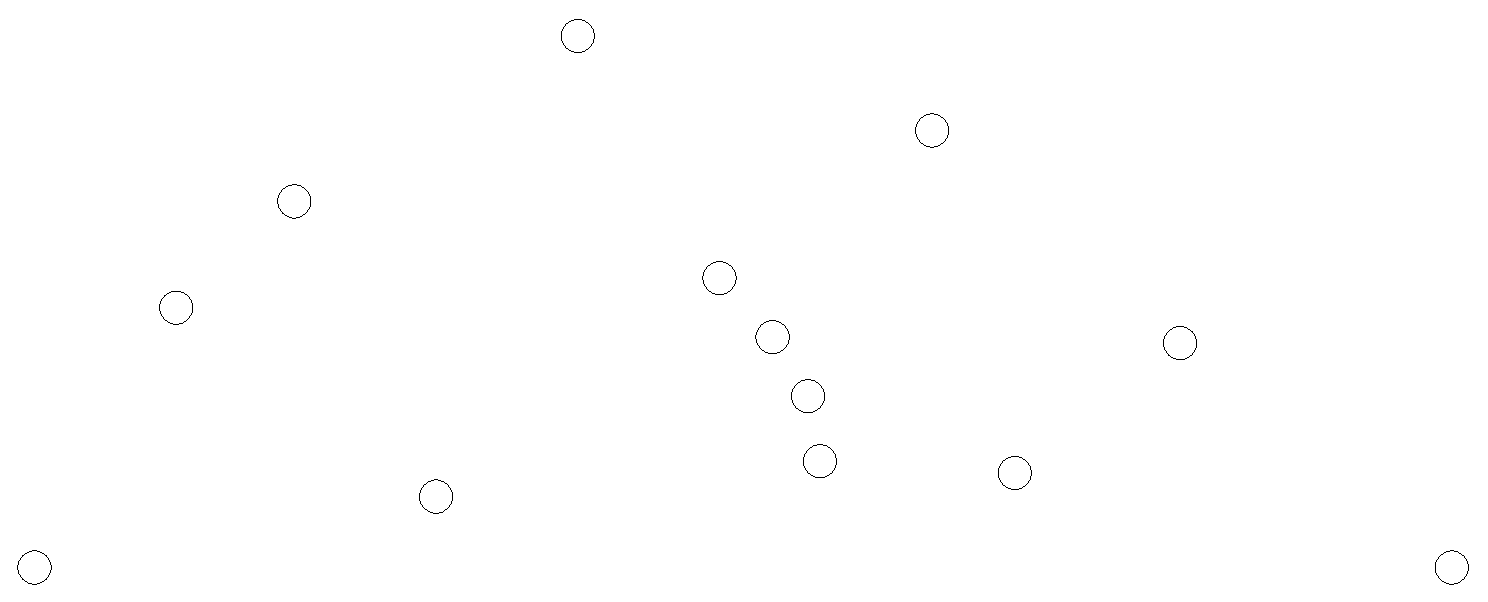
\includegraphics[width=\textwidth]{points}
  \begin{enumerate}
  \item Compute the point $m$ of median $x$-coordinate;
  \item Partition the points by $m.x$;
  \item Compute the highest edge $(a,b)$ intersecting the line $x=m.x$;
  \item Recurse on each side;
  \end{enumerate}
\end{frame}

\subsection{$O(n\lg h)$ in 3D}
\begin{frame}
  \frametitle{2d Convex Hull in $O(n\lg h)$ in 3D}
  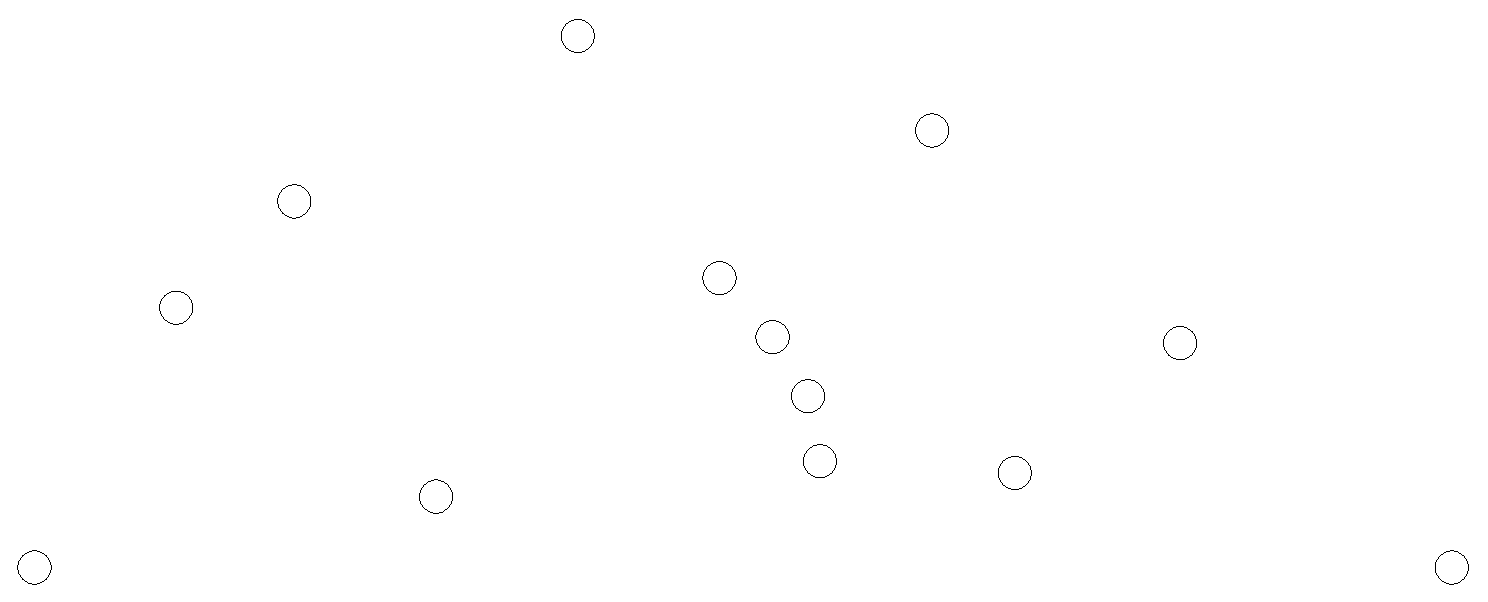
\includegraphics[width=\textwidth]{points}
  \begin{enumerate}
  \item Start with a small guess for $h$;
  \item Group the instances in $n/h$ $x$-sorted groups of size $h$;
  \item Simulate the $O(nh)$ algorithms on the groups;
  \item If it did not suffice, merge the group two by two and iterate.
  \end{enumerate}
\end{frame}

\subsection{$O(n H(C))$, instance optimal}

\begin{frame}
  \frametitle{Convex Hull in $O(n(1+H(C)))$}
  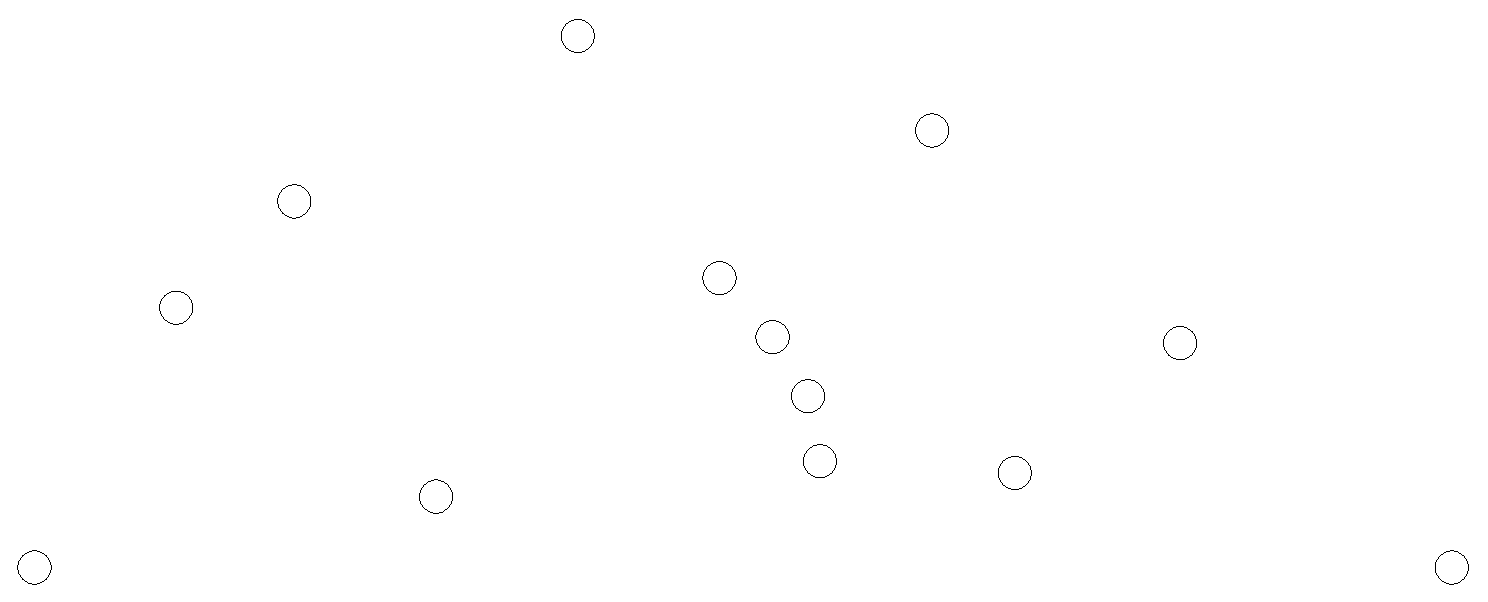
\includegraphics[width=\textwidth]{points}
  \begin{itemize}
  \item Algorithm: a variant of [Kirkpatrick, Seidel]
    \begin{enumerate}
    \item Compute the points leftmost $l$ and rightmost $r$;
    \item Compute the point $m$ of median $x$-coordinate;
    \item Compute the highest edge $(a,b)$ intersecting the line $x=m.x$;
    \item Remove all points contained in the polygon $(l,a,b,r)$;
    \item Recurse on each side;
    \end{enumerate}
  \end{itemize}
\end{frame}

\begin{frame}
  \frametitle{Instance Optimality: definitions}
  
  \begin{definition}[Instance Optimality]
    An algorithm is \alert{instance-optimal} if its cost is at most a
    constant factor from the cost of any other algorithm $A'$ running on
    the same input, for {\em every} input instance.
  \end{definition}
  
  Unfortunately, for many problems, this requirement is too stringent. 
  
  \begin{definition}[Input Order Oblivious Instance Optimality]
    For a set $S$ of $n$ elements in ${\cal D}$, let $T_A(S)$ denote
    the maximum running time of $A$ on input $\sigma$ over all $n!$
    possible permutations $\sigma$ of $S$.  Let $\OPT(S)$ denote the
    minimum of $T_{A'}(S)$ over all correct algorithms $A'\in\A$.  If
    $A\in\A$ is a correct algorithm such that $T_A(S)\le
    O(1)\cdot\OPT(S)$ for every set $S$, then we say $A$ is
    \alert{instance-optimal in the order-oblivious setting}.
  \end{definition}
\end{frame}

\begin{frame}
  \frametitle{Certificate and Instance Optimal Proof}
  \begin{definition}[Certificate]
    A \emph{Certificate} for an instance $I$ and a solution $S$ is the
    description of a sequence of steps to \alert{check} the validity
    of $S$ for $I$.
  \end{definition}
  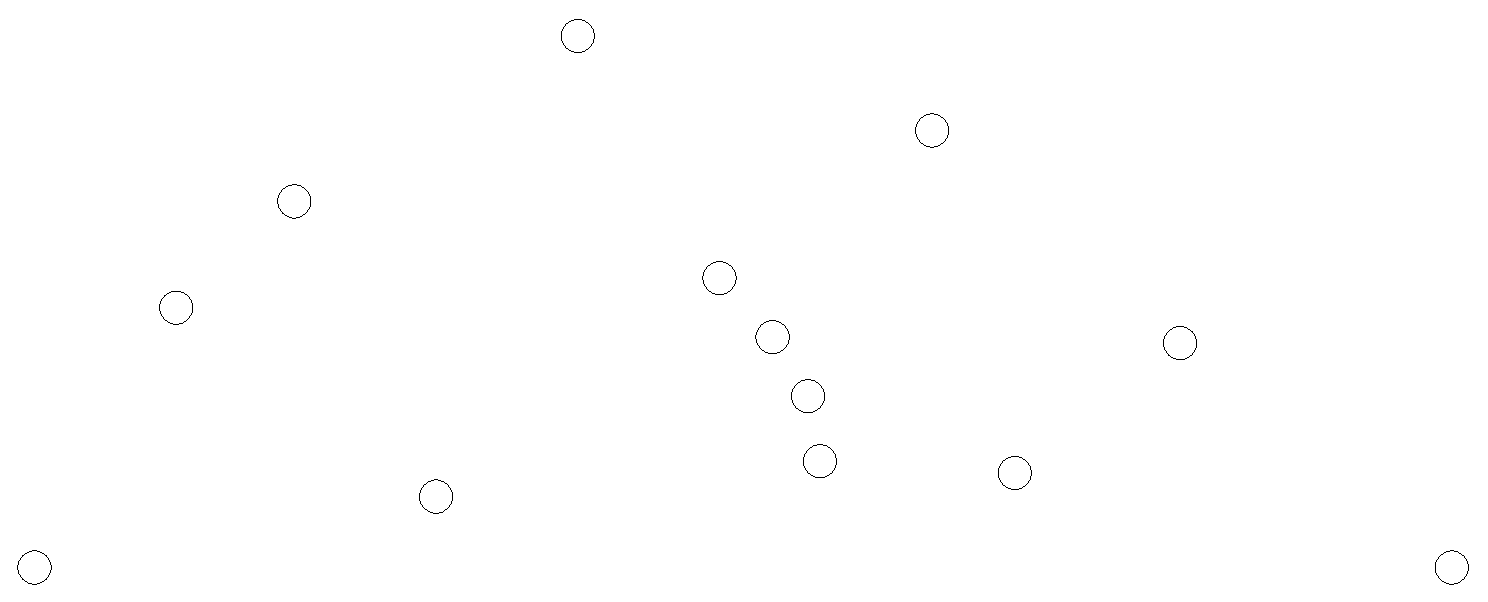
\includegraphics[width=\textwidth]{points}
  \begin{example}
    For the convex hull, a list of triangles and the points they
    cover.
  \end{example}
\end{frame}


\section{Similar Paradoxes}

\begin{frame}<handout>
  \frametitle{Similar Paradoxes}
  \begin{itemize}
  \item Optimal Prefix Free Codes [{Closed to linear in word-RAM}]
  \item Optimal Minimax Trees [{Semi Closed to linear in word-RAM}]
  \item Optimal Alphabetic Binary Search Tree [\alert{Open}]
  \item Directed Max $(s,t)$ Flow [\alert{Open}]
  \item Undirected Min $(s,t)$ Cut [\alert{Semi Open}]
  \item I am looking for more!
  \end{itemize}
\end{frame}

%\subsection{Prefix Free Codes and variants}

\begin{frame}
  \frametitle{Optimal Prefix Free Codes [In Progress]}
  \begin{itemize}
  \item $O(n\lg n)$ classical algorithm.
  \item $O(n)$ algorithm when frequencies are sorted.
  \item $O(n)$ algorithm when frequencies are all within a factor of $2$.
  \item $O(n)$ algorithm when frequencies are all distinct by factor of $2$.
  \item Adaptive Results for $k$ distinct code lengths:
    \begin{itemize}
     \item Belal and Elmasry claim $O(nk)$ in STACS 2006. 
     \item Belal and Elmasry claim $O(n 4^k)$ in ARXIV 2012.
     \end{itemize}
  \item A lower bound of $\Omega(n\lg k)$ in the worst case over
  instances resulting in $k$ distinct code lengths.
\item Conjectures:
  \begin{itemize}
  \item $O(n\lg k)$ adaptive algorithm?
  \item $O(nH(n_1,\ldots,n_k))$ instance optimal algorithm?
  \item $O(n)$ algorithm in word-RAM?
  \end{itemize}
  \end{itemize}
\end{frame}

\begin{frame}
  \frametitle{Optimal Minimax Trees [Open]}
  \begin{itemize}
  \item Tree minimizing the max weight+height of a leaf.
  \item $O(n\lg n)$ classical algorithm [Golumbic];
  \item $O(n)$ algorithm when weights partially sorted by fractional part [Drmota, Szpankowski];
  \item $O(nd\lg\lg n)$ where $d$ is the number of distinct values
    $\lceil w_i\rceil$ [Kirkpatrick and Klawe]
  \item $O(n)$ algorithm in word-RAM [Gawrichowski,Gagie]!
  \end{itemize}
\end{frame}

\begin{frame}
  \frametitle{Optimal Alphabetic Binary Search Tree [Open]}
  \begin{itemize}
  \item $O(n\lg n)$ classical Hu-Tucker algorithm;
  \item $o(n\lg n)$ algorithms in many particular cases;
  \item $O(n)$ algorithm when frequencies ``can be sorted in linear time'';
  \item A lower bound of $\Omega(n\lg k)$ in the worst case over
    instances resulting in $k$ distinct code lengths.
  \end{itemize}
\end{frame}

\begin{TOKEEPSECRET}
%  \subsection{Planar Graph Algorithms}
  \begin{frame}
    \frametitle{Directed Max $(s,t)$ Flow [Open]}
    \begin{itemize}
    \item $O(n\lg n)$ classical algorithm;
    \item $O(n)$ well known algorithm when $s$ and $t$ share a face;
    \item $O(nk)$ new algorithm, where $k$ is the number of edges
      between $s$ and $t$;
    \end{itemize}
  \end{frame}

  \begin{frame}
    \frametitle{Undirected Min $(s,t)$ Cut [Semi Open]}
    \begin{itemize}
    \item $O(n\lg n)$ well known algorithm
    \item $O(n\lg k)$ recent algorithm (STACS 2011!)
    \item Can this be improved?
    \end{itemize}
  \end{frame}
\end{TOKEEPSECRET}

\section*{Summary}

\begin{frame}
  \frametitle<presentation>{Summary}

  \begin{itemize}
  \item $O(nk)$ and $O(n\lg n)$ suggests $O(n\lg k)$
  \item and (Input Order Oblivious) \alert{Instance Optimality}.
%  \item more about it in \alert{CC5109-Analisis Fino de Algoritmos y Estructuras de Datos} next semester.
  \end{itemize}
  
  % The following outlook is optional.
  \vskip0pt plus.5fill
  \begin{itemize}
  \item
    Outlook
    \begin{itemize}
    \item Input Order Adaptive Instance Optimality.
    \item Full Instance Optimality (Kolmogorov's complexity?)
    \item $1$-instance optimality!
    \end{itemize}
  \end{itemize}
\end{frame}


\end{document}



%%% Local Variables:
%%% mode: latex
%%% TeX-master: t
%%% End:
